\section{Konfigurationstool der 3D-Portfolios (Content Creation)} \label{Konfigurationstool}
\setauthor{Litzlbauer Lorenz}

Die Content-Creation-Funktion war eine der Kernfunktionen des Projekts. Mit der Content-Creation konnten die 3D-Portfolios erst entstehen. Es galt einen einfachen und intuitiven Konfigurationsprozess für 3D-Portfolios zu gestalten. Im Entwicklungsprozess wurden viele Entscheidungen getroffen, die auf das ganze Projekt Einfluss hatten. Z.B. wurde eine Art der Datenrepräsentation der 3D-Portfolios und die Darstellungsweise der Daten in der 3D-View entwickelt.

In diesem Kapitel wird die Entwicklung und das System der Content Creation erklärt.

\begin{figure}[h t]
    \centering
    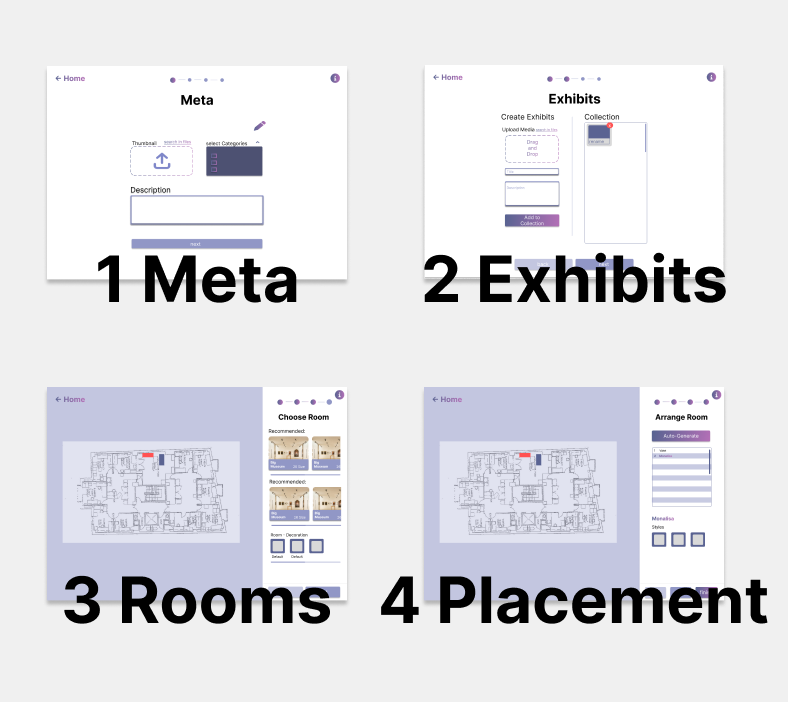
\includegraphics[scale=0.5]{pics/CreateCreation4Categories.png}
    \caption{Die vier Erstellungskategorien}
    \label{fig:impl:creation:fourCategoires}
\end{figure}

\subsection{Überblick}
Das Content-Creation-Tool besteht aus insgesamt vier Unterseiten (siehe Abbildung \ref{fig:impl:creation:fourCategoires}), mit diesen werden Daten gesammelt, um das Portfolio zu erstellen und vielen Untersystemen (Komponenten, Klassen und Services), die beim Erstellungsprozess helfen.

Diese Unterseiten wurden aufgeteilt, damit der*die Benutzer*in sich im Konfigurationsprozess nur mit jeweils einer Portfolio-Daten-Kategorie beschäftigen muss und nicht überfordert wird. Dabei wurde sich  am \emph{Wizard-UI-Pattern} (mehr dazu im Unterkapitel \ref{sec::contentcreation::wizard} auf der Seite \pageref{sec::contentcreation::wizard}) orientiert.

\subsection{Userinterface-Struktur / Wizard Design Pattern}
\label{sec::contentcreation::wizard}
Im Projekt wurde das Wizard-UI-Pattern benutzt, um den Konfigurationsprozess des Portfolios einfacher zu gestalten. Dafür wurden die Konfigurationsdaten nach 4 Kategorien aufgeteilt.

Die Kategorien sind (siehe Abbildung \ref{fig:impl:creation:fourCategoires}):
\begin{compactitem}
\item Metadaten - Die Metadaten sind Daten, die das Portfolio beschreiben, dazu gehören Name, zugehörige Kategorien, eine Beschreibung und ein Thumbnail.
\item Ausstellungsstück - Die Daten des Ausstellungsstücks bestehen aus den vom User auf den Server geladenen Kunstwerken und Zusatzinformation wie Namen und Beschreibung.
\item Raumdaten - Raumdaten bestehen aus den virtuellen 3D-Daten des Raumes und weiteren Konfigurationsdaten wie den Positionen, an denen Ausstellungsstücke im Raum platziert werden können.
\item Ausstellungsplatzierungsdaten - Mit diesen Daten werden die Daten zu den Ausstellungsstücken und dem virtuellen Raum logisch verbunden.
\end{compactitem}

\subsubsection*{Begriffserklärung}
Der Begriff "\emph{Wizard}", in der Softwareentwicklung, kommt ursprünglich von Systemadministratoren, welche bei komplizierten Installationsprozessen halfen oder ganz übernahmen. Mit der Zeit änderte sich der Begriff zu Software-Assistenten-Programmen, welche dem*der User*in dabei unterstützten, die Software zu konfigurieren. \cite[Ursprung des Begriffs Wizard]{OrigionOfWizards}

\subsubsection{Wizard-UI-Pattern}
In dem Web-Bereich gibt es in der Regel zwei Arten, Dateneintragungen zu verarbeiten.

Formulare und Wizards. Virtuelle Formulare sind dabei ähnlich aufgebaut wie reale Formulare, in denen die Formularfelder ausgeführt werden sollen. Hingegen ist ein Wizard eine eigene kleine Applikation, die den*die Benutzer*in durch eine Folge von Formularen führt und gegebenenfalls beim Ausfüllen unterstützt. Je nach den Eingaben können Wizards die Reihenfolge oder die Formulare ändern.

TODO: bei Bedarf könnte hier mehr geschrieben werden. \cite[Wizards: Definition and Design Recommendations]{WizradsDefinitionAndRecommandation}

\subsubsection{Implementation}
Für die Implementation des Wizards wurde die Angular Material Komponente Mat-Stepper benutzt. Sie bietet eine solide Basis für den Wizard. Content kann sequentiell dargestellt werden, während dem*der User*in der aktuelle Status des Wizards durch eine Navigationsleiste angezeigt wird (siehe Abbildung \ref{fig:impl:creation:mathorziontalstepper}). \cite{amStepper}

\begin{figure}[h t]
    \centering
    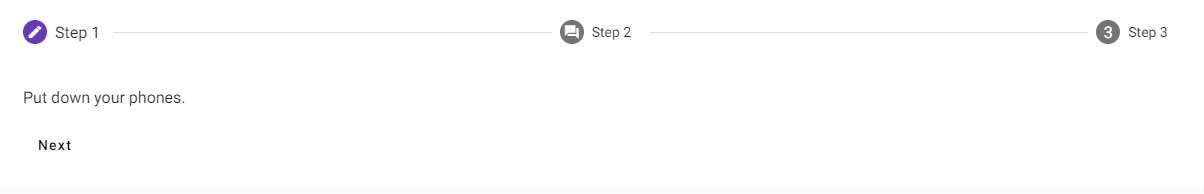
\includegraphics[scale=0.5]{pics/mathorziontalstepper.png}
    \caption{Angular Material: horizontaler Stepper \cite{amStepper}}
    \label{fig:impl:creation:mathorziontalstepper}
\end{figure}

\subsection{4 Formularunterseiten}
Nachdem die Angular Material Komponente Mat-Stepper gewählt wurde, war der nächste Schritt, die vier Formularunterseiten des Wizards (siehe Abbildung \ref{fig:impl:creation:fourCategoires}) zu gestalten.


\subsection{Unterstützende Services und Klassen}